\documentclass[conference]{IEEEtran}

% -------------------------------------------------
% Packages
% -------------------------------------------------
\usepackage{amsmath,amssymb}
\usepackage{graphicx}
\usepackage{booktabs}
\usepackage{array}
\usepackage{url}
\usepackage{cite}
\usepackage{microtype}

\graphicspath{{diagrams/}{./}}

% -------------------------------------------------
% Document
% -------------------------------------------------
\begin{document}

% -------------------------------------------------
% Title
% -------------------------------------------------
\title{AI-Driven Automated Interview Platform with Avatar-Based Candidate Assessment}

% -------------------------------------------------
% Authors
% -------------------------------------------------
\author{
\IEEEauthorblockN{
Shlok Abhishek,
Satyadip Lal,
Mannat,
Aditya Raj
}
\IEEEauthorblockA{
3rd Year Students, Department of CSE\\
School of Engineering and Technology\\
Sharda University, Greater Noida, Uttar Pradesh, India
}
\and
\IEEEauthorblockN{
V. Sathiyasuntharam
}
\IEEEauthorblockA{
Mentor, Department of CSE\\
School of Engineering and Technology\\
Sharda University, Greater Noida, Uttar Pradesh, India\\
sathiya4196@gmail.com
}
}

\maketitle

% -------------------------------------------------
% Abstract
% -------------------------------------------------
\begin{abstract}
The expansion of asynchronous hiring has created demand for interview systems that scale efficiently without sacrificing candidate engagement or evaluation consistency. This paper presents \textit{AI Interview Platform}, a web-based recruitment ecosystem that enables human resource teams to conduct automated asynchronous video interviews through a personalized AI avatar. The platform pairs a React single-page frontend with a serverless backend and implements a dual-mode evaluation framework: an instruction-tuned large language model (LLM) generates questions and evaluates open-ended responses semantically, while a deterministic rule-based engine acts as an immediate fallback whenever external connectivity is disrupted. A key architectural feature is the synthesis of an interviewer avatar from an HR professional's photographs and voice profile, synchronized with text-to-speech (TTS) and real-time speech-to-text (STT) for conversational delivery. To uphold assessment integrity without transmitting private video streams, the platform includes a client-side morphological computer vision heuristic that detects unauthorized mobile phone consultation directly on HTML5 Canvas buffers. We describe the system architecture, the 3NF normalized database schema, the five-dimension scoring formulation (relevance, accuracy, confidence, keyword coverage, and professional skill signals), and the graceful degradation strategy. We report a functional evaluation of the implemented platform and examine its alignment with emerging statutory standards for automated hiring tools, including NYC Local Law 144, the Illinois Artificial Intelligence Video Interview Act, and the European Union AI Act.
\end{abstract}

% -------------------------------------------------
% Index Terms
% -------------------------------------------------
\begin{IEEEkeywords}
Artificial Intelligence, Large Language Models, Automated Video Interviewing, Synthetic Avatars, Speech Recognition, Candidate Assessment, Graceful Degradation, Edge Computer Vision, Algorithmic Fairness
\end{IEEEkeywords}

% -------------------------------------------------
% I. INTRODUCTION
% -------------------------------------------------
\section{Introduction}

High-volume talent acquisition remains an operational bottleneck in modern organizations. When applicant volume increases, recruiters face significant hurdles in maintaining evaluation consistency, minimizing turnaround times, and delivering an engaging candidate experience \cite{cappelli,levashina}. Conventional unstructured interviews are susceptible to interviewer subjectivity, fatigue, and grading disparities \cite{salgado}. While structured interviews reduce variance, organizing them across multiple candidates and interviewers remains resource-intensive.

Recent advances in natural language processing (NLP) and large language models (LLMs) allow systems to generate context-aware questions and evaluate spoken answers semantically \cite{devlin,brown}. However, many existing automated screening tools present applicants with static text forms or chatbots. This lack of interpersonal cues can make the evaluation feel impersonal, discouraging candidates and obscuring verbal communication dynamics \cite{bauer}.

To address this, we developed \textit{AI Interview Platform}, a web-based system that combines automated interview workflows with a personalized AI avatar. An avatar trained on an interviewer's photographs and voice samples delivers questions through text-to-speech synthesis, while candidates respond verbally and visually through browser media APIs. The system automates session creation, question generation, candidate registration, response recording, multi-dimensional scoring, and ranking.

At the same time, automated hiring platforms face growing regulatory and legal scrutiny. Concerns regarding algorithmic bias, disability accommodations, and transparency have led to significant legal actions and statutory frameworks \cite{hirevue,aclu}. New York City Local Law 144 requires annual independent bias audits and impact-ratio reporting for automated employment decision tools \cite{nyclaw}. The Illinois Artificial Intelligence Video Interview Act mandates candidate disclosure, explanation, and consent \cite{illinois}. The EU AI Act classifies employment-related AI systems as high-risk, imposing strict transparency and human-oversight duties \cite{euaiact}. This regulatory context directly informs our design choices regarding candidate consent, data minimization, and human-in-the-loop decision boundaries.

\begin{figure*}[!t]
    \centering
    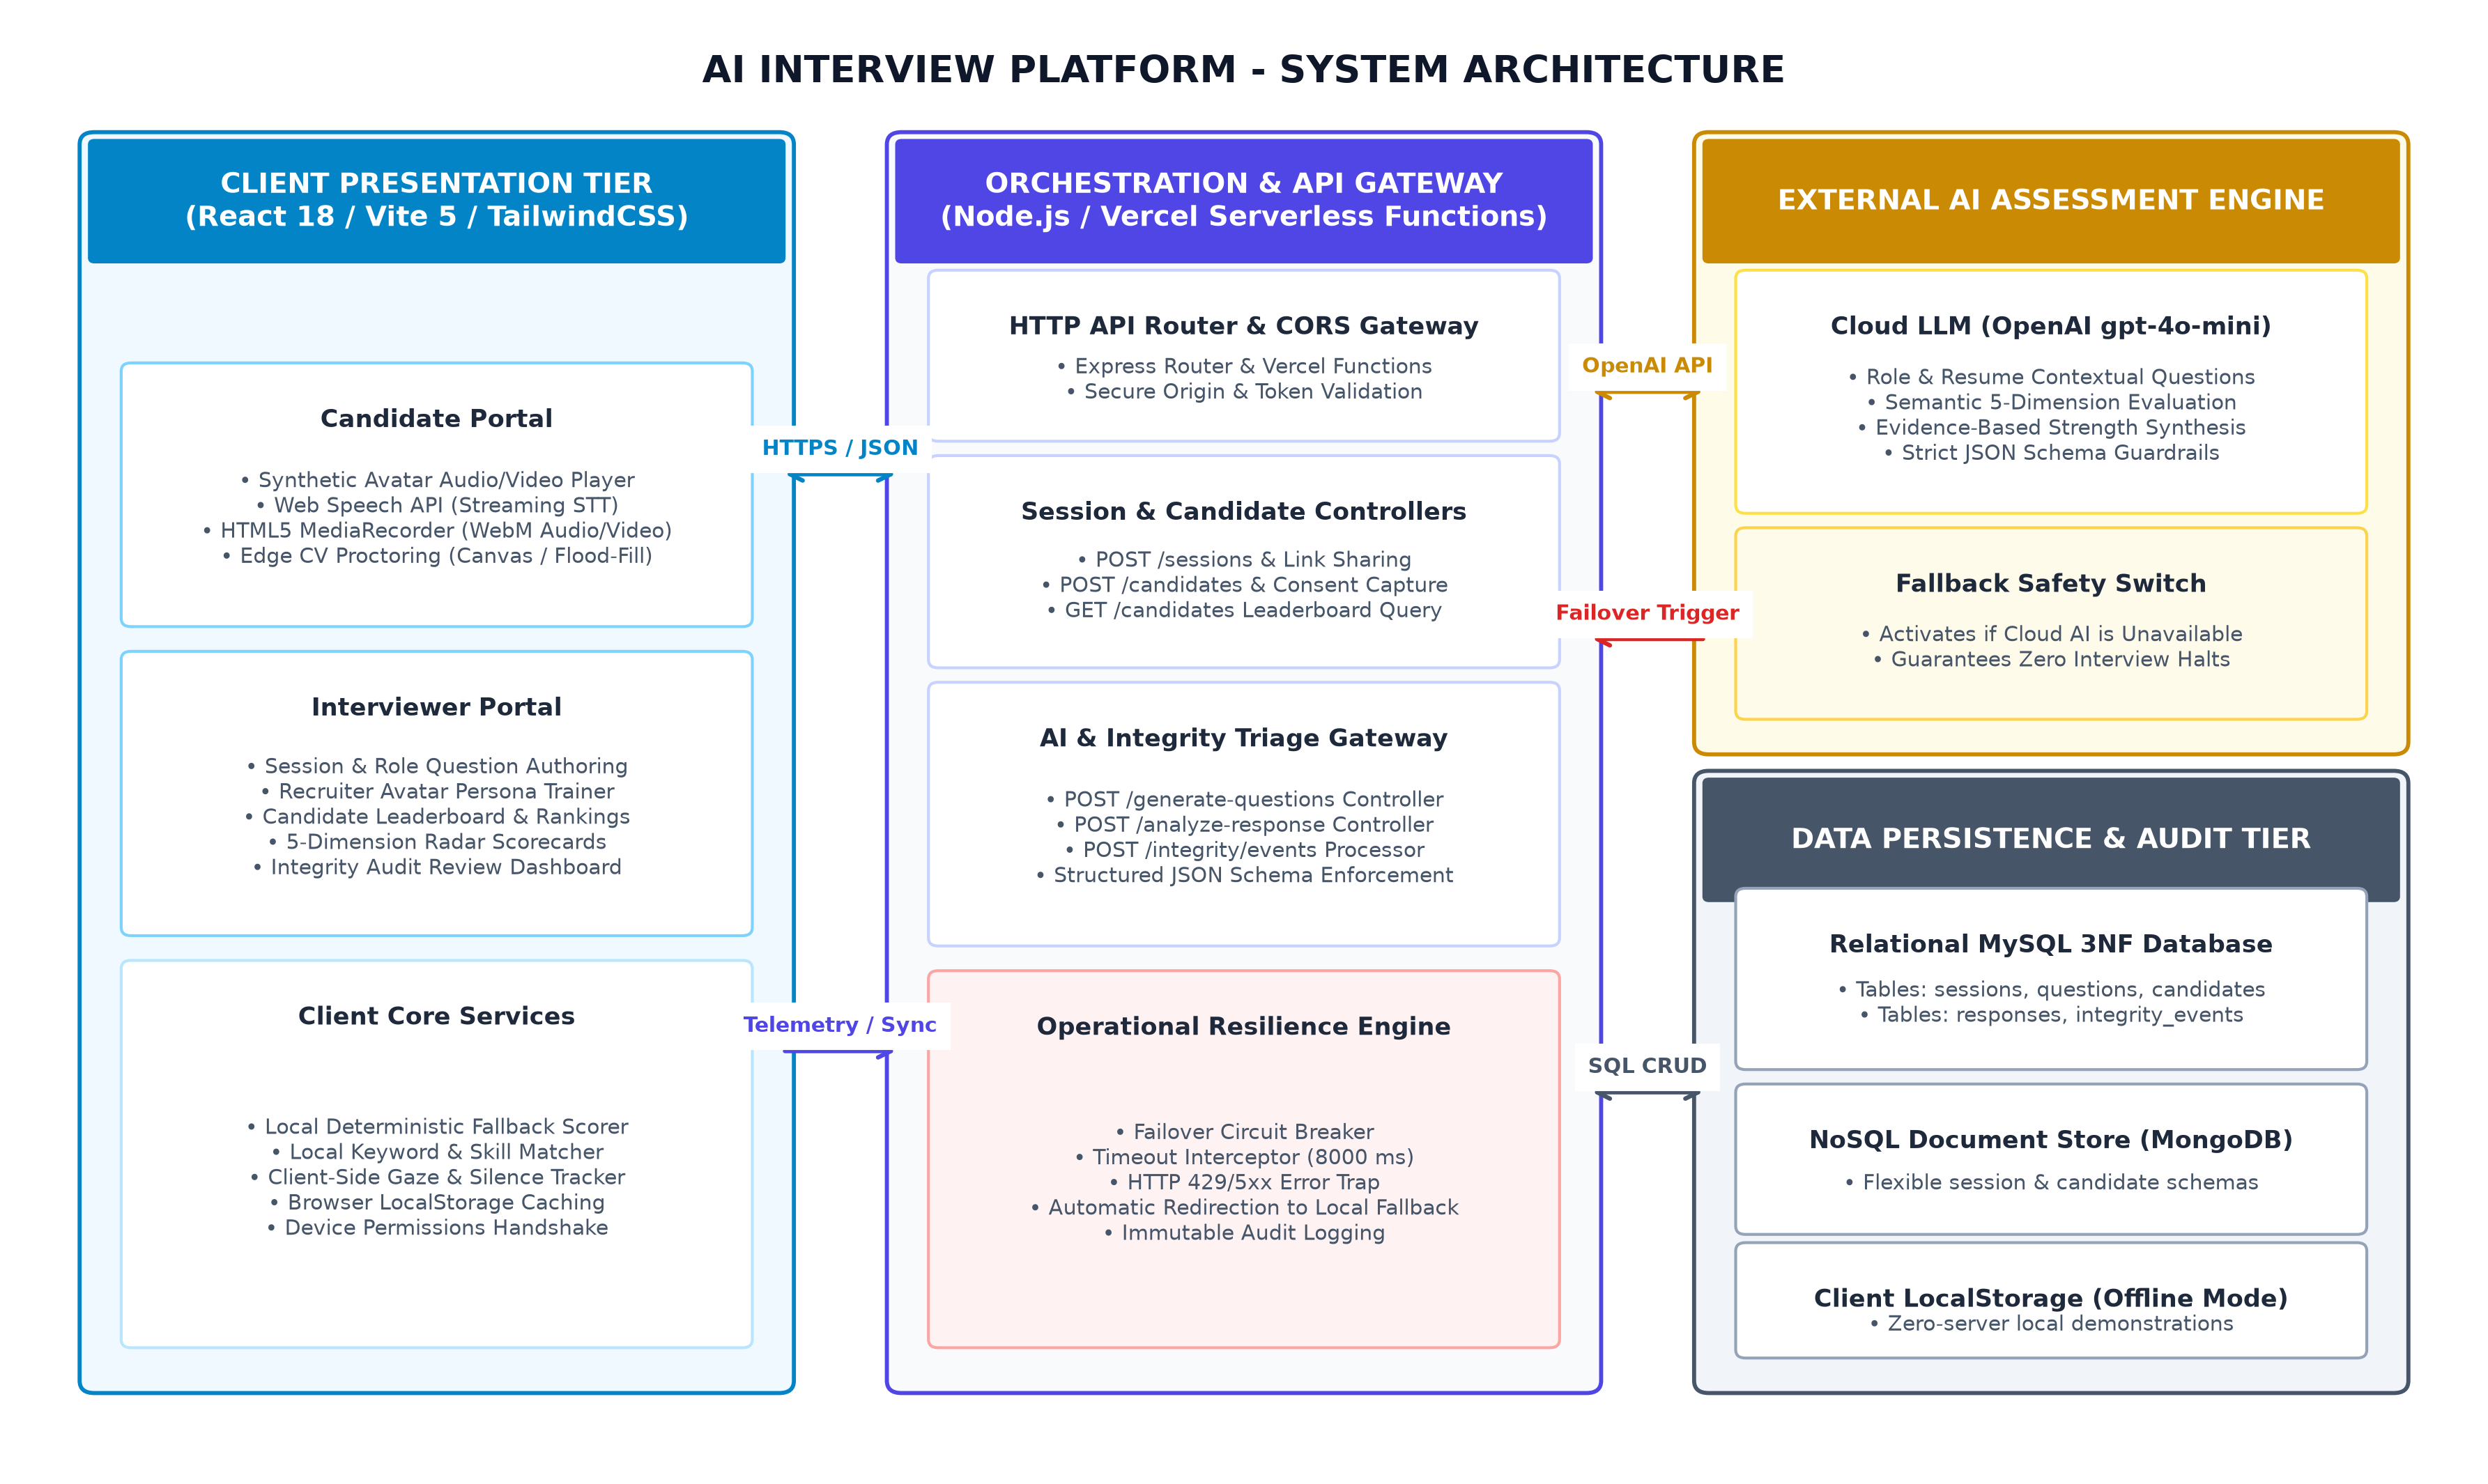
\includegraphics[width=0.92\textwidth]{system_architecture.png}
    \caption{End-to-end architectural topology of the AI Interview Platform. The client frontend comprises dedicated portals for candidates and interviewers, executing edge-based speech synthesis, streaming transcription, and morphological proctoring. The serverless orchestration layer coordinates cloud-based LLM response evaluation with an automatic failover circuit breaker that transparently engages an on-device deterministic scoring engine during API latency spikes or outages.}
    \label{fig:architecture}
\end{figure*}

The primary contributions of this paper are as follows:
\begin{itemize}
    \item We design and implement a full-stack, serverless-ready architecture featuring role-segregated portals for corporate interviewers and applicants, backed by a 3NF normalized persistence tier.
    \item We propose a personalized synthetic avatar pipeline pairing recruiter likeness with neural text-to-speech (TTS) audio narration and visual speech state changes.
    \item We develop a dual-mode question generation and response scoring framework that executes deep semantic evaluation via instruction-calibrated LLMs while guaranteeing continuous platform availability through a local deterministic fallback engine.
    \item We formulate a multi-dimensional assessment rubric evaluating answers along five quantifiable axes: relevance ($R$), technical accuracy ($A$), linguistic confidence ($C$), keyword coverage ($K$), and professional competency presence ($S$).
    \item We implement a privacy-preserving, edge-computed morphological computer vision heuristic that detects unauthorized handheld smartphone usage on client canvas buffers without streaming raw imagery to external servers.
    \item We conduct a functional evaluation verifying the operational behavior of the implemented modules, and detail architectural alignment with NYC Local Law 144, Illinois 820 ILCS 42, and the EU AI Act.
\end{itemize}

The remainder of this paper is organized as follows. Section II reviews related work and regulatory contexts. Section III describes the system architecture. Section IV details the core methodology and scoring formulation. Section V describes implementation specifics and user interfaces. Section VI presents functional evaluation and verification results. Section VII discusses ethical and regulatory alignment. Section VIII concludes the paper and outlines future directions.

% -------------------------------------------------
% II. RELATED WORK
% -------------------------------------------------
\section{Related Work and Regulatory Context}

\subsection{Automated Interview Evaluation}

Early automated interview systems relied on predefined question banks and rule-based keyword intersection \cite{salgado}. While computationally efficient, these systems could not capture semantic intent or reward synonymous technical phrasing. Transformer models such as BERT \cite{devlin} and instruction-tuned autoregressive LLMs \cite{brown} have enabled semantic similarity scoring and contextual answer understanding. Our platform builds on this foundation by deploying instruction-tuned LLMs with strictly validated JSON schemas, while retaining a deterministic scoring engine as an operational fail-safe.

\subsection{Avatars and Virtual Agents}

Text-to-speech and computer-vision techniques have enabled conversational agents in education and customer service \cite{sridhar,cassell}. However, the use of personalized avatars trained on specific recruiters within asynchronous hiring remains relatively uncommon. Our platform pairs avatar personalization with real-time browser-based speech processing to enhance applicant presence without prohibitive streaming render costs.

\subsection{Regulatory Landscape}

Commercial automated interview tools have faced major challenges regarding transparency and fairness. A 2019 FTC complaint against HireVue prompted the vendor to remove facial-analysis scoring in 2021 \cite{hirevue}. In 2023, the EEOC settled a landmark algorithmic discrimination suit involving automated age screening \cite{eeoc}. More recently, legal complaints have highlighted the necessity of accessible accommodation protocols for candidates with speech or hearing impairments \cite{aclu}. Regulatory mandates such as NYC Local Law 144 \cite{nyclaw}, the Illinois AI Video Interview Act \cite{illinois}, and the EU AI Act \cite{euaiact} require advance candidate disclosure, auditable evaluation metrics, and mandatory human oversight, which we treat as baseline system design requirements.

% -------------------------------------------------
% III. SYSTEM ARCHITECTURE
% -------------------------------------------------
\section{System Architecture}

The system architecture follows a decoupled client-server model designed for scalability and resilience, as illustrated in Fig.~\ref{fig:architecture}. The frontend is a React single-page application, while the backend consists of serverless API endpoints and a relational persistence layer.

\subsection{Frontend Presentation Tier}

The user interface layer is built with React 18, Vite 5, and TailwindCSS 3, organized into two dedicated portals:
\begin{itemize}
    \item \textbf{Interviewer Portal:} allows recruiters to create sessions, define job requirements, author or auto-generate questions, configure avatar likeness, inspect response recordings, examine candidate scores, and review integrity logs.
    \item \textbf{Candidate Portal:} accessible via unique session links, guides applicants through device verification, informed consent, avatar question delivery, real-time transcription, and response recording.
\end{itemize}

\subsection{Serverless Orchestration Gateway}

The backend tier is architected as lightweight serverless micro-functions deployed on Vercel infrastructure, supplemented by a Node.js development runtime. The gateway provides secure RESTful endpoints for session lifecycle operations, question authoring, resume feature extraction, candidate scoring, and integrity telemetry aggregation. Crucially, the gateway encapsulates all external AI credentials within server-side execution boundaries. It incorporates an automated circuit breaker that intercepts third-party service latency anomalies ($> 8000\text{ ms}$) or HTTP $429/5xx$ status codes, redirecting evaluation requests to the deterministic fallback engine without client interruption.

\subsection{Data Persistence and Schema Topology}

The platform supports dual-mode persistence:
\begin{enumerate}
    \item \textbf{Local-First Browser Persistence:} Utilizes the Web Storage API to cache session states, candidate responses, and proctoring telemetry on client devices, enabling zero-configuration offline demonstrations.
    \item \textbf{Relational MySQL 3NF Database:} Integrates with a normalized MySQL database structured in Third Normal Form (3NF) enforcing foreign-key constraints across six core tables: \texttt{interviewer}, \texttt{session}, \texttt{question}, \texttt{candidate}, \texttt{response}, and \texttt{integrity\_event}, ensuring referential integrity and supporting immutable audit trails required for statutory compliance.
\end{enumerate}

\begin{table}[htbp]
\caption{System Technology Stack}
\label{tab:technology}
\centering
\renewcommand{\arraystretch}{1.2}
\begin{tabular}{p{0.34\columnwidth}p{0.58\columnwidth}}
\toprule
\textbf{Subsystem Layer} & \textbf{Component Implementation and Role}\\
\midrule
Client Framework & React 18, Vite 5, TailwindCSS 3 (Modular UI)\\
State \& Routing & Context API, React Router 6, Lucide React\\
Speech Synthesis & Web Speech API (\texttt{SpeechSynthesisUtterance})\\
Speech Recognition & Web Speech API (\texttt{webkitSpeechRecognition})\\
Media Pipeline & HTML5 MediaRecorder (VP8/Opus WebM)\\
Edge Computer Vision & HTML5 Canvas, Morphological Flood-Fill Engine\\
Primary AI Engine & OpenAI API (\texttt{gpt-4o-mini} with JSON Schemas)\\
Fallback Analyzer & Local Deterministic Rule-Based Scorer\\
Gateway Runtime & Node.js, Vercel Serverless Functions\\
Persistence Engine & MySQL (3NF Normalized), MongoDB, LocalStorage\\
\bottomrule
\end{tabular}
\end{table}

% -------------------------------------------------
% IV. METHODOLOGY
% -------------------------------------------------
\section{Methodology and Algorithmic Formulation}

\subsection{Personalized AI Avatar}

HR professionals upload facial photographs and optional video clips to configure the avatar. During an interview, the avatar displays the interviewer's likeness while question text is narrated using browser-native text-to-speech. Rate and pitch parameters are tuned for natural delivery:
\begin{equation}
\nu_{\text{rate}} = 0.95 \cdot \nu_{\text{base}}, \quad \rho_{\text{pitch}} = 1.02 \cdot \rho_{\text{base}}
\end{equation}

Visual state transitions are synchronized with utterance execution events. When the TTS engine triggers \texttt{onboundary} or \texttt{onstart} callbacks, the client UI executes subtle CSS transformation matrices and animates active-speaking status auras, conveying dynamic presence. When speech concludes, the avatar transitions gracefully into a passive attentive posture. Candidates are provided with interface controls to replay questions, adjust audio output, and toggle subtitles.

\subsection{Dual-Mode Question Generation Pipeline}

Interview inquiries can be synthesized through two operational pathways:
\begin{itemize}
    \item \textbf{Generative LLM Synthesis:} When connected to external services, the serverless gateway constructs an instruction-tuned prompt concatenating the target job description, required seniority level, and candidate resume extract. The model returns a structured JSON payload defining questions with assigned time allocations ($T_i \in [60, 180]\text{ s}$), domain evaluation rubrics, and expected technical keywords ($\kappa_i$).
    \item \textbf{Deterministic Rule-Based Extraction:} Under disconnected or degraded operational states, an on-device text analyzer applies regular-expression tokenization and keyword extraction across the job specification and resume text. It identifies core competency clusters and instantiates parameterized templates, guaranteeing continuous session authoring.
\end{itemize}

\subsection{Multi-Dimensional Psychometric Scoring Formulation}

Responses are evaluated across five orthogonal dimensions:

\subsubsection{Relevance ($R$)}
Measures semantic congruence between candidate answer text $a$ and question $q$ via lexical overlap with an elaboration bonus:
\begin{equation}
R = \min\left(100, \; \frac{|\mathcal{W}(a) \cap \mathcal{W}(q)|}{|\mathcal{W}(q)|} \times 80 + \beta_{\text{len}}(a)\right)
\end{equation}
where $\mathcal{W}(\cdot)$ extracts unique content words with character length exceeding 3, and $\beta_{\text{len}}(a)$ rewards adequate elaboration ($20$ pts for $30-200$ words, $10$ pts for $20-29$ words).

\subsubsection{Technical Accuracy ($A$)}
Combines keyword coverage ($K$) and relevance ($R$):
\begin{equation}
A = \min(100, \; \text{round}(0.60 \cdot K + 0.40 \cdot R))
\end{equation}

\subsubsection{Linguistic Confidence ($C$)}
Evaluates applicant assertiveness by parsing positive certainty markers against hesitation patterns:
\begin{equation}
C = \text{clamp}\left(50 + 10 \cdot N_{\text{pos}}(a) - 10 \cdot N_{\text{neg}}(a) + \delta_{\text{len}}(a), \; 0, \; 100\right)
\end{equation}
where $N_{\text{pos}}$ tallies assertive phrases, $N_{\text{neg}}$ tallies equivocation markers, and $\delta_{\text{len}}$ provides a bounded adjustment reflecting discursive fluency.

\subsubsection{Keyword Match Ratio ($K$)}
Reflects normalized coverage of expected technical concepts $\kappa$:
\begin{equation}
K = \text{round}\left(\frac{|\kappa \cap \text{lexemes}(a)|}{|\kappa|} \times 100\right), \quad |\kappa| > 0
\end{equation}

\subsubsection{Professional Skill Presence ($S$)}
Quantifies competency keywords across six domains: Communication ($S_1$), Problem Solving ($S_2$), Teamwork ($S_3$), Leadership ($S_4$), Technical Depth ($S_5$), and Adaptability ($S_6$):
\begin{equation}
S_j = \min\left(100, \; \text{round}\left(\frac{|\mathcal{D}_j \cap \text{lexemes}(a)|}{|\mathcal{D}_j|} \times 200\right)\right)
\end{equation}

\subsubsection{Composite Score Integration}
The per-question overall score combines the primary dimensions via normalized empirical weights, scaled by question importance $W_i$:
\begin{equation}
\label{eq:overall_score}
\text{Score}_i = \min\left(100, \; w_R R + w_A A + w_C C + w_K K\right) \cdot W_i
\end{equation}
with empirical weights $w_R = 0.25$, $w_A = 0.30$, $w_C = 0.20$, and $w_K = 0.25$. The qualitative competency vector $\mathbf{S} = [S_1, \dots, S_6]$ is preserved alongside the numerical score.

\begin{figure}[!t]
\centering
\fbox{
\begin{minipage}{0.95\columnwidth}
\small
\textbf{Algorithm 1: Scoring with Resilient Fallback}
\vspace{4pt}
\hrule
\vspace{4pt}
\textbf{Input:} Transcript $a$, question $q$, keywords $\kappa$, weight $W$, skill lexicons $\{\mathcal{D}_j\}_{j=1}^6$.\\
\textbf{Output:} $(\text{Score}, R, A, C, K, \mathbf{S}, \text{evidence})$.
\begin{enumerate}
    \itemsep=2pt
    \item Initialize $\text{isScored} \leftarrow \text{False}$.
    \item \textbf{if} $\text{CircuitBreaker}.\text{isOpen}() == \text{False}$ \textbf{then}
    \begin{enumerate}
        \item $\mathcal{J}_{\text{res}} \leftarrow \text{RemoteLLMScoring}(a, q, \kappa, \text{Schema})$.
        \item \textbf{if} $\mathcal{J}_{\text{res}}$ satisfies schema and bounds \textbf{then}
        \item \quad Extract $R, A, C, K, \mathbf{S}, \text{evidence} \leftarrow \mathcal{J}_{\text{res}}$.
        \item \quad $\text{isScored} \leftarrow \text{True}$.
        \item \textbf{end if}
    \end{enumerate}
    \item \textbf{if} $\text{isScored} == \text{False}$ \textbf{then}
    \begin{enumerate}
        \item $R \leftarrow \text{ComputeRelevance}(a, q)$ via Eq. (2).
        \item $K \leftarrow \text{ComputeKeywordCoverage}(a, \kappa)$ via Eq. (5).
        \item $A \leftarrow \text{ComputeAccuracy}(K, R)$ via Eq. (3).
        \item $C \leftarrow \text{ComputeConfidence}(a)$ via Eq. (4).
        \item $\mathbf{S} \leftarrow \{\text{ComputeSkillPresence}(a, \mathcal{D}_j)\}_{j=1}^6$ via Eq. (6).
        \item $\text{evidence} \leftarrow \text{SynthesizeRuleBasedNotes}(a, \kappa, \mathbf{S})$.
    \end{enumerate}
    \item $\text{Score} \leftarrow \min(100, \; w_R R + w_A A + w_C C + w_K K) \cdot W$.
    \item \textbf{return} $(\text{Score}, R, A, C, K, \mathbf{S}, \text{evidence})$.
\end{enumerate}
\vspace{2pt}
\end{minipage}
}
\caption{Operational logic of the multi-dimensional scoring engine with automated failover.}
\label{alg:scoring}
\end{figure}

\subsection{Client-Side Phone-Usage Detection}

To preserve interview integrity while respecting candidate privacy, the platform implements a client-side computer vision heuristic operating on downsampled HTML5 Canvas frames (scanned every $\Delta t_{\text{scan}} = 1500\text{ ms}$). Candidate pixels are flagged if matching phone chassis or screen profiles:
\begin{equation}
\mathcal{P}(x,y) \iff \left(\bar{I} < 55\right) \lor \left(\bar{I} > 185 \;\land\; \Delta_{\text{RGB}} < 38\right)
\end{equation}
where mean luminance $\bar{I} = \frac{R + G + B}{3}$ and chromatic spread $\Delta_{\text{RGB}} = \max(R,G,B) - \min(R,G,B)$.

Contiguous candidate pixels are aggregated into spatial components using 4-connectivity flood fill. For each bounding box of dimensions $W_b \times H_b$ and pixel count $\Omega$, aspect ratio $\psi$ and rectangularity factor $\phi$ are computed:
\begin{equation}
\psi = \frac{\max(W_b, H_b)}{\max(1, \min(W_b, H_b))}, \quad \phi = \frac{\Omega}{\max(1, W_b \cdot H_b)}
\end{equation}

An unauthorized device alert is flagged when $\Omega_{\min} \le \Omega \le \Omega_{\max}$, $1.45 \le \psi \le 3.8$, $\phi > 0.42$, and normalized vertical center $\bar{Y}_{\text{norm}} > 0.18$, with confidence:
\begin{equation}
\Lambda_{\text{phone}} = \min\left(0.92, \; 0.70 \cdot \phi + 0.20 \cdot \min(\psi, 2.8)\right)
\end{equation}

When $\Lambda_{\text{phone}} \ge 0.58$, an advisory warning is displayed and logged with a 5000 ms cooldown. Concurrently, audio energy is monitored to flag extended silences ($E_{\text{rms}} < 0.035$ for $> 3500\text{ ms}$). Video frames are never sent to remote servers.

\begin{figure}[!t]
    \centering
    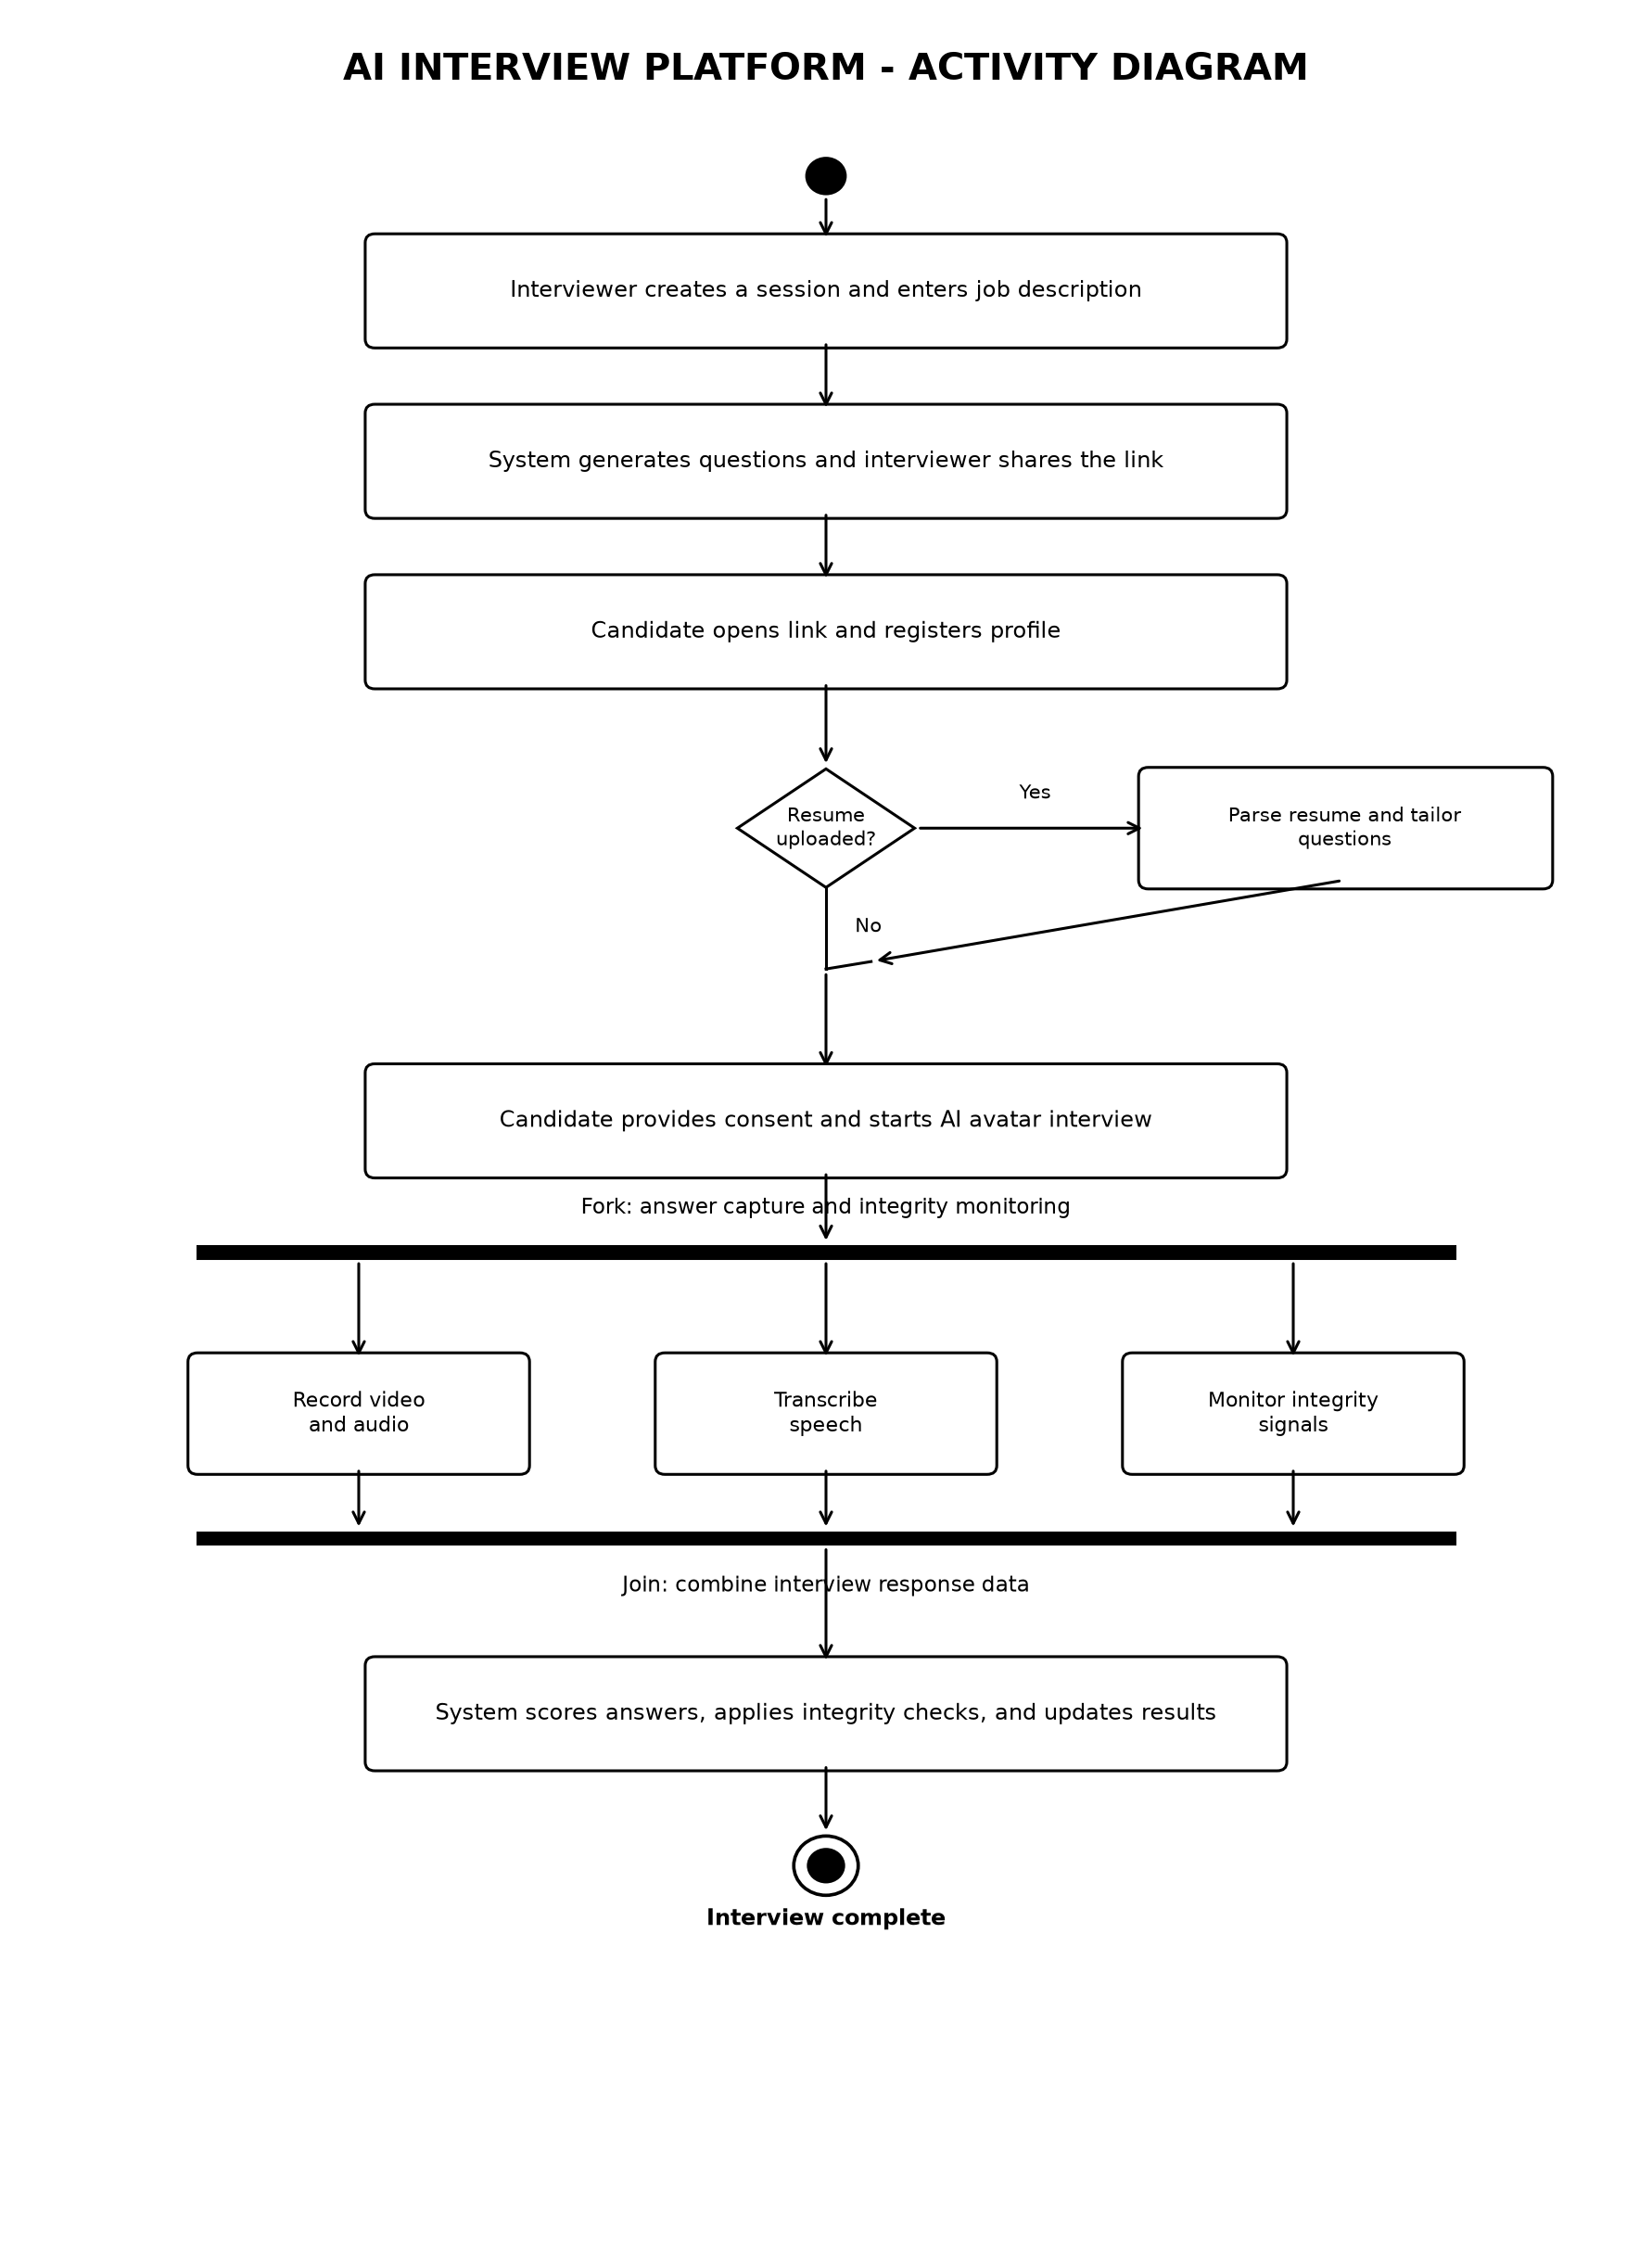
\includegraphics[width=0.88\columnwidth]{diagram_activity_perfect.png}
    \caption{UML Activity Diagram of the AI Interview Platform, showing the complete end-to-end execution flow: session initialization, question generation, candidate registration, avatar-conducted interview, concurrent capture of video, audio transcription, and integrity heuristics, followed by response scoring and candidate completion.}
    \label{fig:activity}
\end{figure}

% -------------------------------------------------
% V. IMPLEMENTATION
% -------------------------------------------------
\section{Implementation and User Interfaces}

The system is implemented as a full-stack JavaScript application using React 18, Vite 5, TailwindCSS 3, and Node.js. Vocal answers are captured using the MediaRecorder API as WebM audio/video blobs, while the browser SpeechRecognition interface generates streaming transcripts. All network communications are encrypted via HTTPS, and API keys are isolated server-side.

Fig.~\ref{fig:usecase} illustrates the platform's functional use cases, modeling the end-to-end actor relationships across the Interviewer, Candidate, AI Service, and Integrity Service. Fig.~\ref{fig:classdiag} details the corresponding UML Class Diagram, defining entity relationships and service boundaries across the architecture.

\begin{figure*}[!t]
    \centering
    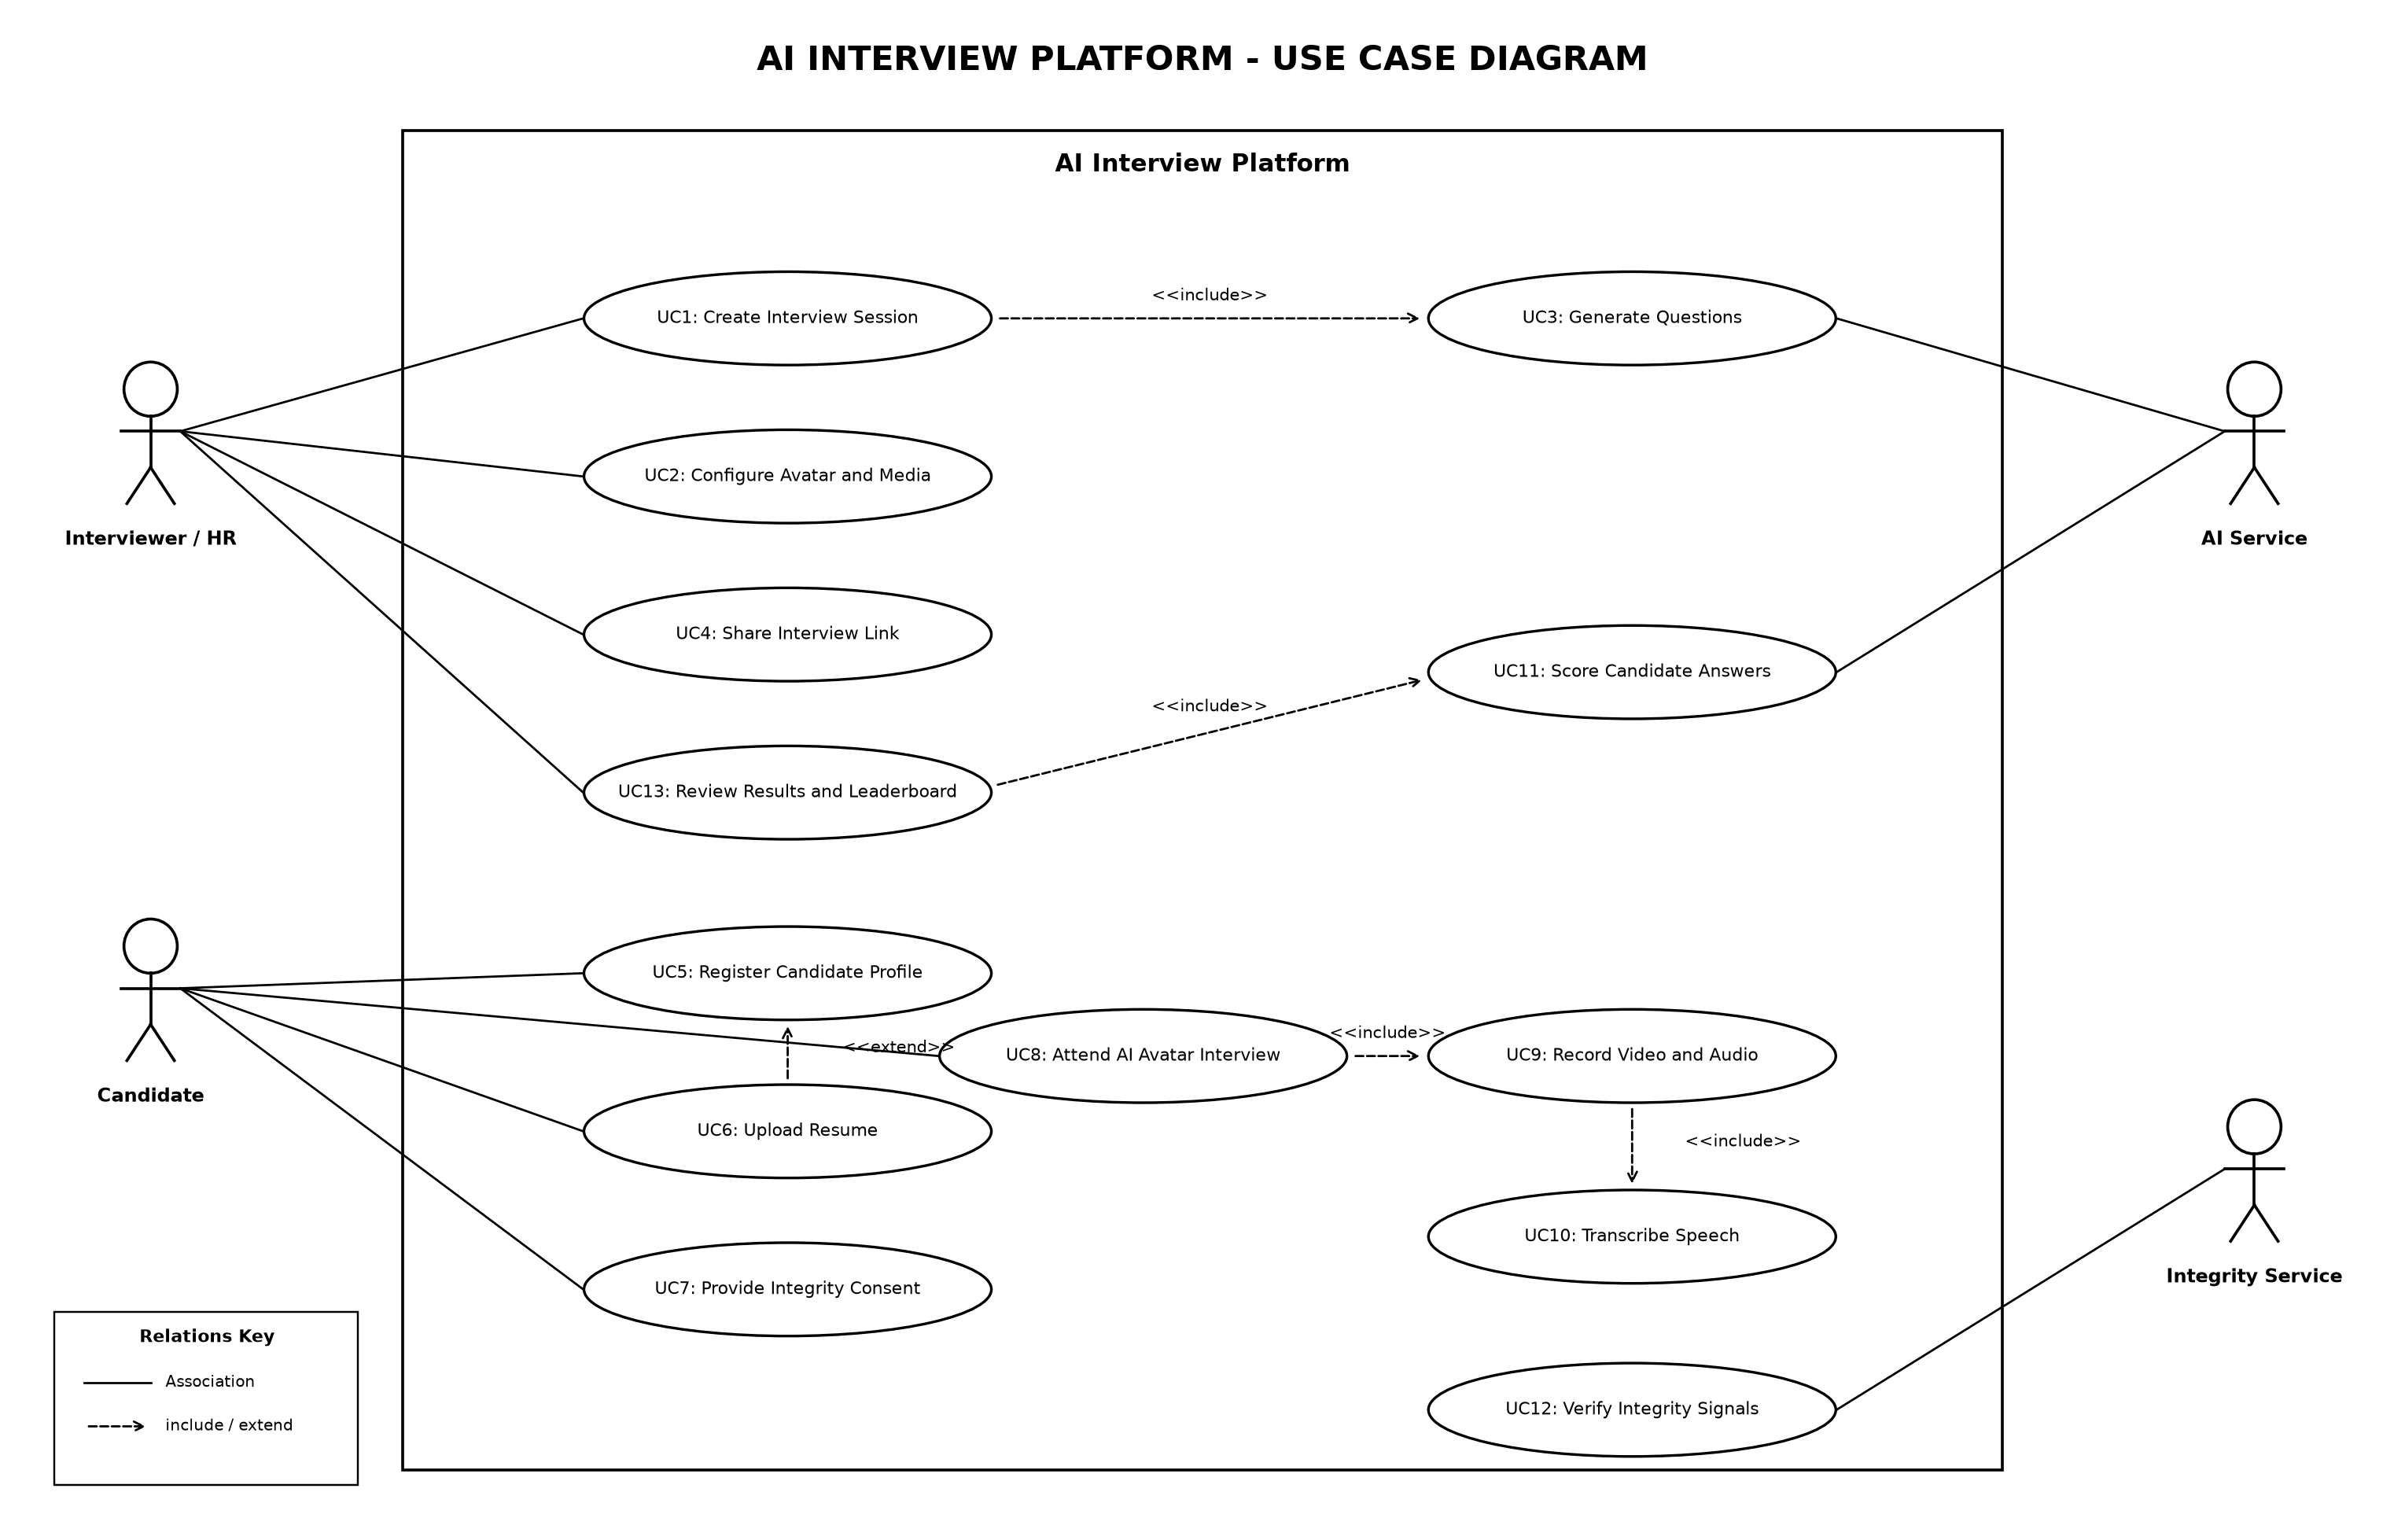
\includegraphics[width=0.92\textwidth]{diagram_usecase_perfect.png}
    \caption{UML Use Case Diagram of the AI Interview Platform, modeling interactions among the four primary actors (Interviewer/HR, Candidate, AI Service, and Integrity Service) across 13 core operational use cases (UC1 through UC13), including automated session management, AI question generation, avatar delivery, streaming transcription, edge proctoring, and auditable candidate scoring.}
    \label{fig:usecase}
\end{figure*}

\begin{figure*}[!t]
    \centering
    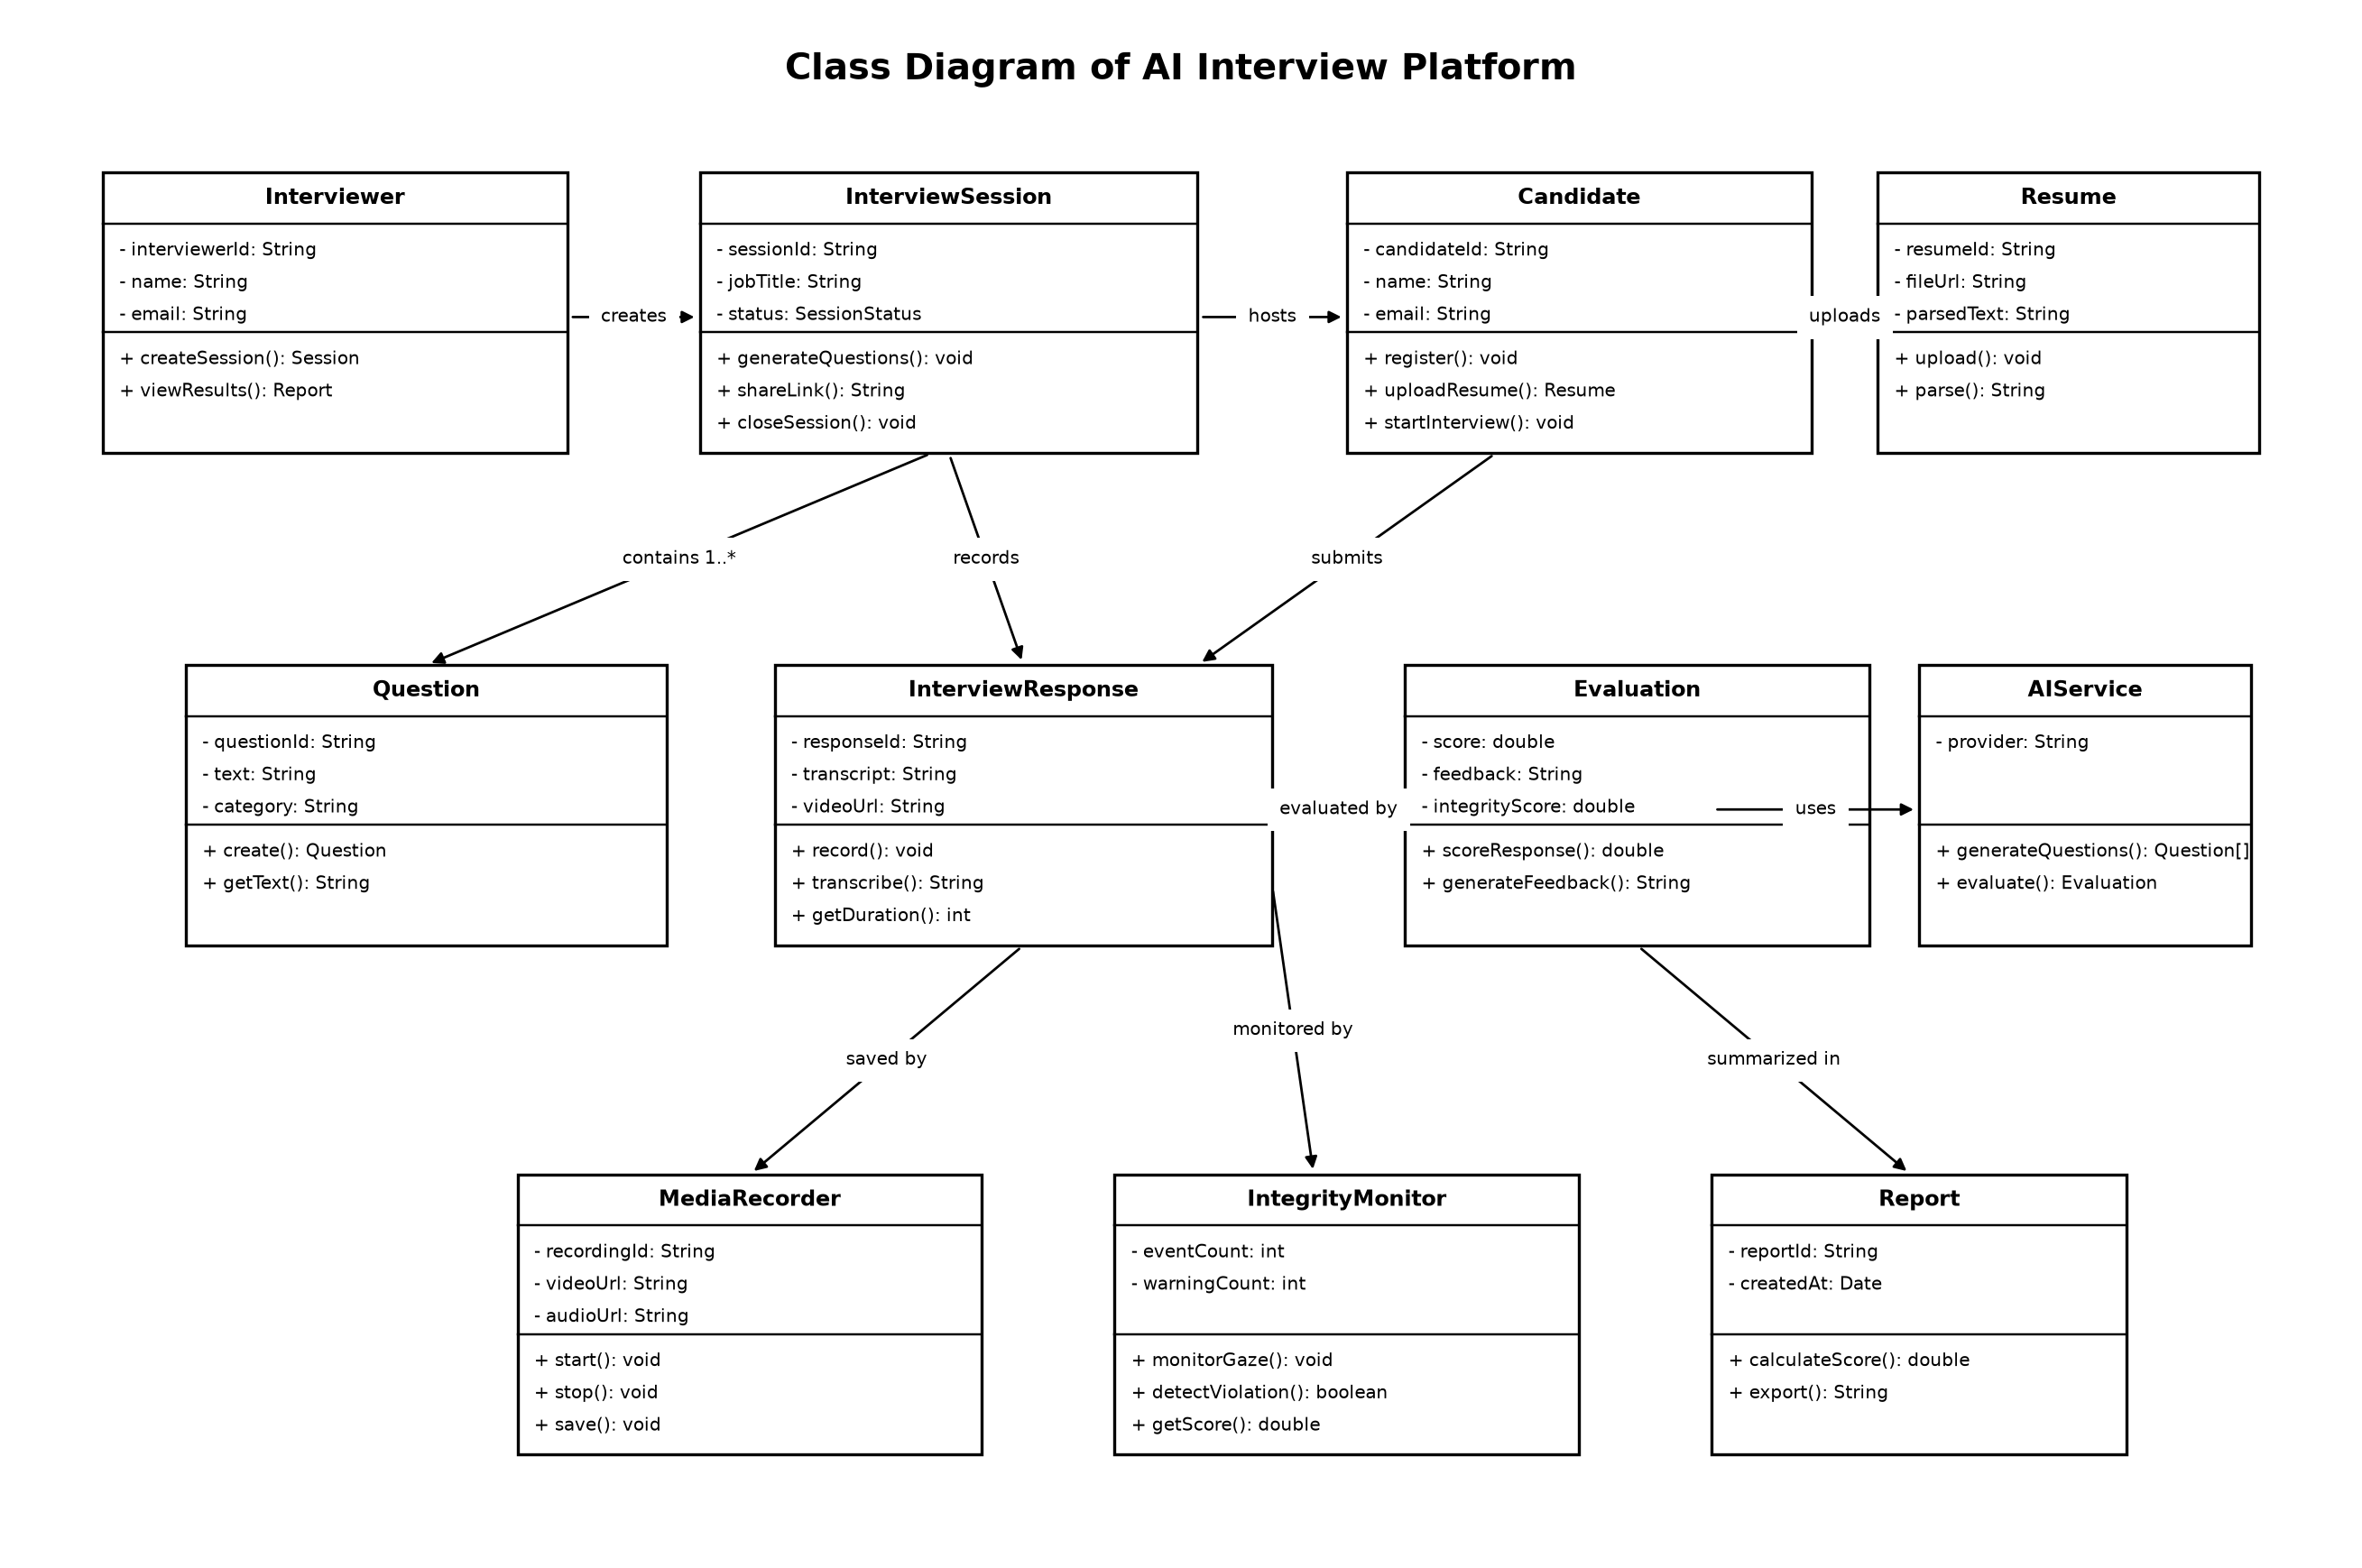
\includegraphics[width=0.88\textwidth]{uml_class_diagram_ai_interview_platform.png}
    \caption{UML Class Diagram detailing the object-oriented structure of the platform, showing relationship dependencies between portal controllers, session entities, speech and proctoring services, and the multi-dimensional scoring engine.}
    \label{fig:classdiag}
\end{figure*}

% -------------------------------------------------
% VI. EVALUATION
% -------------------------------------------------
\section{Functional Evaluation and System Verification}

\subsection{Functional Testing of Platform Modules}

We evaluated the platform across both interviewer and candidate workflows. Table~\ref{tab:verification} summarizes the verification results for the core functional modules. The avatar system guided candidates through multi-question sessions with synchronized audio narration and visual speech state changes. Real-time transcription operated reliably in Chromium-based browsers, producing usable transcripts for immediate scoring. Both question-generation pathways functioned as designed: the AI-assisted mode produced role-relevant questions from job descriptions, while the local deterministic mode extracted skills and generated structured questions without external internet connectivity.

\begin{table}[htbp]
\caption{Functional Verification of Core Modules}
\label{tab:verification}
\centering
\renewcommand{\arraystretch}{1.2}
\begin{tabular}{p{0.28\columnwidth}p{0.44\columnwidth}c}
\toprule
\textbf{Module} & \textbf{Verification Test} & \textbf{Status}\\
\midrule
Avatar Narration & Photo upload + TTS narration & Pass\\
Speech STT & Live streaming transcription & Pass\\
AI Question Gen & Role \& JD prompt synthesis & Pass\\
Fallback Gen & Offline skill/project extraction & Pass\\
5D Scorer & $R, A, C, K, S$ score calculation & Pass\\
Phone Detection & Connected-component CV heuristic & Pass\\
Audio Anomaly & Silence floor threshold detection & Pass\\
3NF Persistence & MySQL relational table CRUD & Pass\\
\bottomrule
\end{tabular}
\end{table}

\subsection{Scoring Resilience and Fallback Behavior}

Under normal operating conditions, the LLM provides nuanced evaluation narratives and calibrated scores. When network interruptions or API errors were simulated, the circuit breaker automatically engaged the deterministic scorer without aborting candidate sessions. The deterministic engine provides consistent, reproducible baseline scores ($\sigma^2 = 0$ across identical inputs), ensuring operational continuity.

\subsection{Edge Proctoring Observations}

The connected-component phone-detection heuristic reliably detected high-contrast rectangular objects during active recording. Because the heuristic relies on morphological features and thresholding, lighting variations can cause false positives. Consequently, integrity events are recorded as advisory review telemetry for human recruiters rather than automated disqualifications.

\subsection{Limitations}

Several limitations are noted: (1) Speech recognition accuracy varies across browsers, operating best in Chrome and less reliably in Safari and Firefox; (2) The deterministic fallback scorer is bounded by literal keyword matching and cannot reward synonyms; (3) The phone-detection heuristic is sensitive to camera placement and lighting; and (4) Third-party LLM rate limits constrain concurrency.

% -------------------------------------------------
% VII. ETHICAL CONSIDERATIONS
% -------------------------------------------------
\section{Ethical Considerations and Regulatory Alignment}

\subsection{Disclosure and Consent (Illinois 820 ILCS 42)}

In compliance with the Illinois Artificial Intelligence Video Interview Act, the platform displays an advance disclosure modal informing candidates that AI is used to generate questions and evaluate responses, requiring explicit consent before initializing media capture.

\subsection{Auditability and Disparate Impact (NYC Local Law 144)}

NYC Local Law 144 mandates annual independent bias audits evaluating selection-rate impact ratios across race and sex. The platform stores granular per-dimension scores and question weights in normalized relational tables, providing structured data for external auditability:
\begin{equation}
AIR = \frac{\text{Selection Rate}_{\text{protected}}}{\text{Selection Rate}_{\text{reference}}} \ge 0.80
\end{equation}

\subsection{Human-in-the-Loop Oversight (EU AI Act)}

In alignment with the EU AI Act's high-risk classification, candidate rankings serve as decision-support signals for recruiters. The system does not execute automated rejections, maintaining mandatory human review for all hiring decisions.

\subsection{Accessibility Accommodations}

To support candidates with disabilities pursuant to ADA Title III, the platform provides subtitle captions, question replay, and audio volume controls, ensuring accessibility for hearing-impaired applicants.

% -------------------------------------------------
% VIII. CONCLUSION
% -------------------------------------------------
\section{Conclusion and Future Work}

We presented \textit{AI Interview Platform}, a web-based automated interview system combining a personalized synthetic avatar, real-time speech processing, dual-mode question generation, and a five-dimension scoring model with a deterministic fallback. The platform demonstrates that engaging asynchronous interviewing can be achieved without complex 3D streaming infrastructure, while maintaining operational resilience during network interruptions. Future work will focus on formal demographic bias audits, improved deep-learning edge object detection, and multimodal evaluation combining vocal prosody with transcript analysis.

% -------------------------------------------------
% REFERENCES
% -------------------------------------------------
\begin{thebibliography}{16}

\bibitem{cappelli}
P. Cappelli,
``Your approach to hiring is all wrong,''
\textit{Harvard Business Review},
vol. 97, no. 3, pp. 48--58, 2019.

\bibitem{levashina}
J. M. Levashina, C. J. Hartwell, F. P. Morgeson, and M. A. Campion,
``The structured employment interview: Narrative and quantitative review of the research literature,''
\textit{Personnel Psychology},
vol. 67, no. 1, pp. 241--293, 2014.

\bibitem{salgado}
J. Salgado and S. Moscoso,
``Validity of structured interviews,''
in \textit{The SAGE Handbook of Personnel Selection and Assessment},
Thousand Oaks, CA: SAGE Publications, 2012, pp. 287--303.

\bibitem{devlin}
J. Devlin, M.-W. Chang, K. Lee, and K. Toutanova,
``BERT: Pre-training of deep bidirectional transformers for language understanding,''
in \textit{Proc. NAACL-HLT},
Minneapolis, MN, 2019, pp. 4171--4186.

\bibitem{brown}
T. B. Brown \textit{et al.},
``Language models are few-shot learners,''
in \textit{Advances in Neural Information Processing Systems (NeurIPS)},
vol. 33, 2020, pp. 1877--1901.

\bibitem{bauer}
T. N. Bauer, T. Truxillo, K. Mack, and C. Costa,
``Applicant reactions to digital recruitment and selection,''
in \textit{The Oxford Handbook of Job Search and Technology},
Oxford, UK: Oxford Univ. Press, 2022, pp. 315--338.

\bibitem{sridhar}
K. R. Sridhar and S. Narayanan,
``Beyond perceptual thresholds: Speech synthesis and virtual agents,''
\textit{IEEE Transactions on Affective Computing},
vol. 11, no. 1, pp. 1--14, 2020.

\bibitem{cassell}
J. Cassell, J. Sullivan, S. Prevost, and E. Churchill,
\textit{Embodied Conversational Agents},
Cambridge, MA: MIT Press, 2000.

\bibitem{hirevue}
K. Harwell,
``A face-scanning algorithm increasingly decides whether you deserve the job,''
\textit{The Washington Post},
Nov. 2019;
Electronic Privacy Information Center,
``EPIC complaint to the FTC in re HireVue,''
Nov. 2019.

\bibitem{aclu}
ACLU of Colorado,
``Discrimination complaint filed with the U.S. Equal Employment Opportunity Commission and Colorado Civil Rights Division regarding AI-driven automated hiring platforms,''
Mar. 2025.

\bibitem{eeoc}
U.S. Equal Employment Opportunity Commission,
``EEOC announces settlement of first landmark algorithmic discrimination suit against iTutorGroup,''
EEOC Press Release,
Aug. 2023.

\bibitem{nyclaw}
New York City Council,
``Local Law 144 of 2021: Automated Employment Decision Tools,''
New York City Administrative Code,
effective Jan. 1, 2023.

\bibitem{illinois}
Illinois General Assembly,
``Artificial Intelligence Video Interview Act,''
820 ILCS 42,
effective Jan. 1, 2020.

\bibitem{euaiact}
European Parliament and Council of the European Union,
``Regulation (EU) 2024/1689 (Artificial Intelligence Act),''
\textit{Official Journal of the European Union},
L 2024/1689, July 2024.

\bibitem{suen}
H.-Y. Suen, K.-E. Hung, and C.-L. Lin,
``Intelligent video interview agent: Development and validation of an asynchronous evaluation tool,''
\textit{Computers in Human Behavior},
vol. 100, pp. 248--258, 2019.

\bibitem{raghavan}
M. Raghavan, S. Barocas, J. Kleinberg, and K. Levy,
``Mitigating bias in algorithmic hiring: Evaluating claims and practices,''
in \textit{Proc. ACM FAccT},
Barcelona, Spain, 2020, pp. 469--481.

\end{thebibliography}

\end{document}
